\chapter{Results and Model Identification}
\section{Identification for One-stage Experiment}

The sample result of experiments can be seen in \fref{fig:one-stage}. The x-axis is the motor torques while y-axis is the external wrenches that are transformed from F/T sensor. The reference value (zero-value) of both axis is taken from pre-contact position. 

\begin{figure}[H]
  \begin{subfigure}[t]{0.5\textwidth}
    \centering
    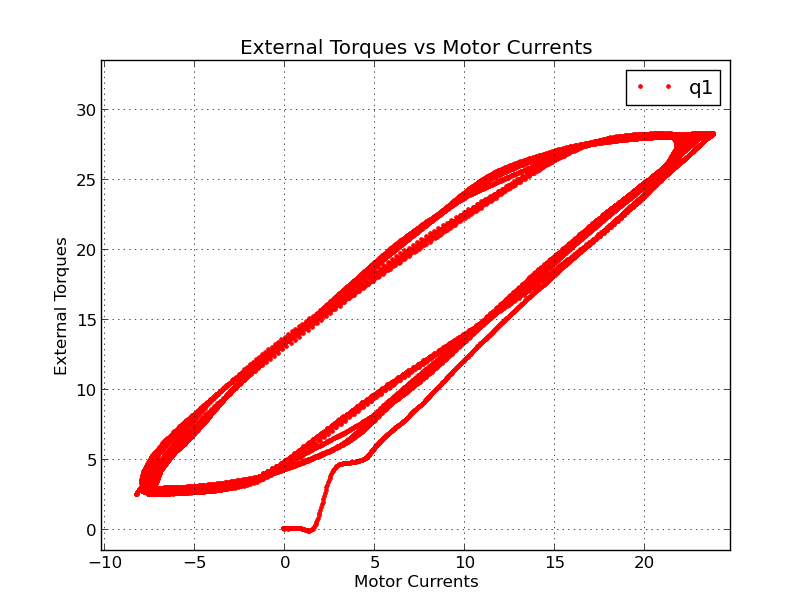
\includegraphics[width = \textwidth ]{fig06} 
    \caption{First joint}
  \end{subfigure}
  \begin{subfigure}[t]{0.5\textwidth}
    \centering
    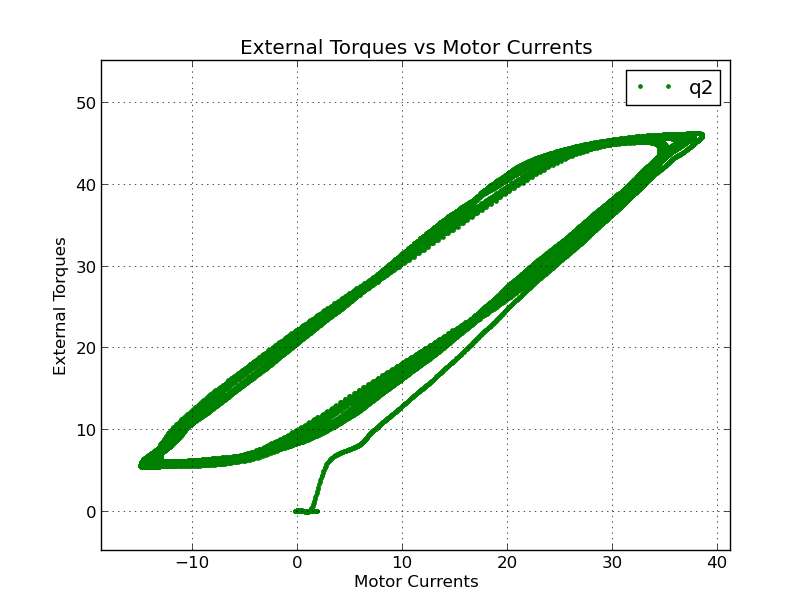
\includegraphics[width = \textwidth ]{fig07}
    \caption{Second joint}
  \end{subfigure}
  \caption{Sample results of one-stage experiment (first two joints)}
  \label{fig:one-stage}
\end{figure}

Firstly, the value for identification is referenced with pre-contact condition. From computation it is known that there is only a few changes in $\tau_{dyn}$ ($\tau_{dyn} = M\left(q\right)\ddot{q} + C\left(\dot{q} , q \right)\dot{q} + G\left(q \right)$) during contact motion and so it can be ommitted. Thus, the dynamic equation can be simplified into just:

\begin{equation}
  J^{T} \Delta F_{ext} = K_{denso} \Delta \tau_{denso} - \tau_{friction} + C
\end{equation}
 
Here a constant is introduced where it is actually a friction during precontact movement, $\tau_{friction,precontact}$. For friction, we will identify it using static friction and Dahl friction. As for Dahl friction, some adjustments to the equation need to be done to match with the optimization. The modified Dahl equation that is going to be used is : 

\begin{align}
  \dot{z} &= p_{2 }\dot{\tau_{mot}} - \left|\dot{\tau_{mot}}\right| p_{3} z \\
  \tau_{friction} &= p_{1} z
\end{align}

To identify all the unknown parameters, the equation is optimized to match with the fitted data. The number of parameters to be optimized will depend on the model of friction that we choose. This optimization is done by using nelder-mead method. One of the result of optimization is shown in \fref{fig:optimization}. It shows the result for both friction model that is going to be used.

 
\begin{figure}[H]
  \begin{subfigure}[t]{0.5\textwidth}
    \centering
    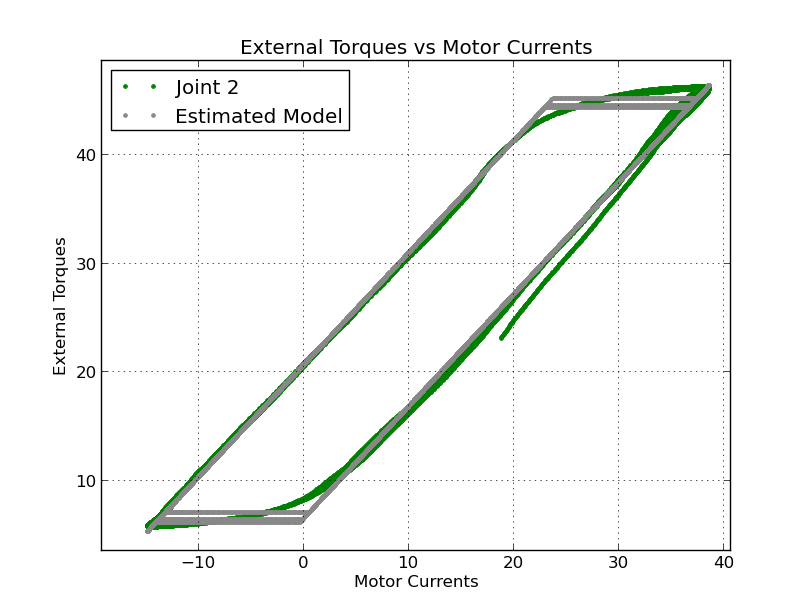
\includegraphics[width = \textwidth ]{fig12} 
    \caption{Using viscous and coulomb model}
  \end{subfigure}
  \begin{subfigure}[t]{0.5\textwidth}
    \centering
    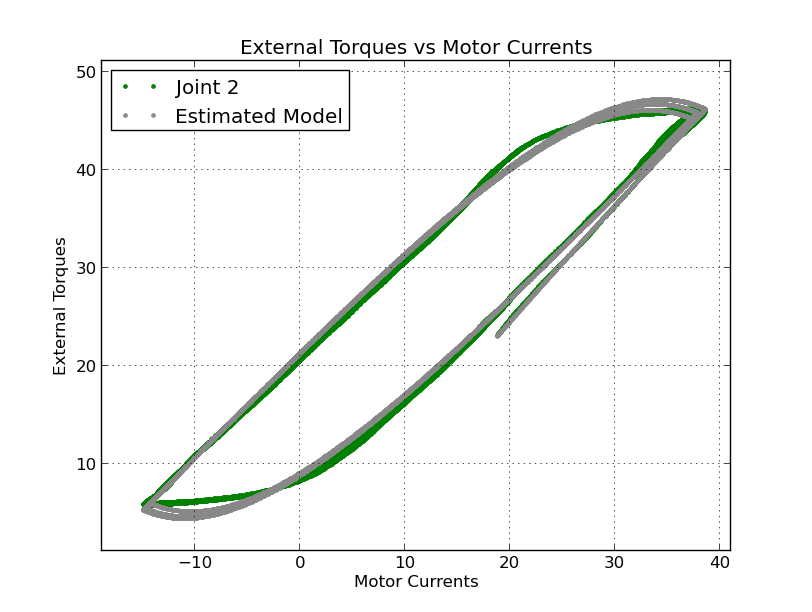
\includegraphics[width = \textwidth ]{fig13}
    \caption{Using Dahl model}
  \end{subfigure}
  \caption{Example of optimization result of one joint (e.g.:second joint)}
  \label{fig:optimization}
\end{figure}

From \fref{fig:optimization}, it is quite clear that the results will depend on the friction model that we choose. Using Dahl model, the error value to the fitted data is less than using coulomb + viscous friction. However, Dahl model imposes one problem. The model requires initial state of $z$. During optimization, this value is unknown and hence it was optimized together with other parameters. However, this initial state will always change for every different position of the arm. Thus, it makes the model more difficult to implement since we need to know the initial state. This will be more clear in the next chapter of validation (see chapter \ref{validation}).

While the identification can be done, it is difficult to distinguish the effect of each parameter, especially between viscous effect and denso gain. Hence, the experiment was then rescheduled using two-stage experiment (see section \ref{two-stage experiment}).

\section{Preliminary Results for Two-stage Experiment}
Two figures below are some samples of the collected data during the experiment. The whole data are available in the appendix. The data has been filtered to eliminate the noise reading available from the sensor or motor. It uses low pass filter for smoothing the result. Low pass filter for F/T sensor have the order of 3 with cutoff frequency of 2 Hz. As for the motor torque, the low pass filter is set to have the order of 5 and cutoff frequency of 1 Hz unless special adjustment is required.

\fref{fig: push result} represents the result of high torque experiment for one of the joint and \fref{fig: fric result} represents the data collected during the free motion experiment. The results from \fref{fig: push result} will be further processed for calibrating the motor torque while results in \fref{fig: fric result} are used for friction identification.

\begin{figure}[H]
  \begin{subfigure}[t]{0.5\textwidth}
    \centering
    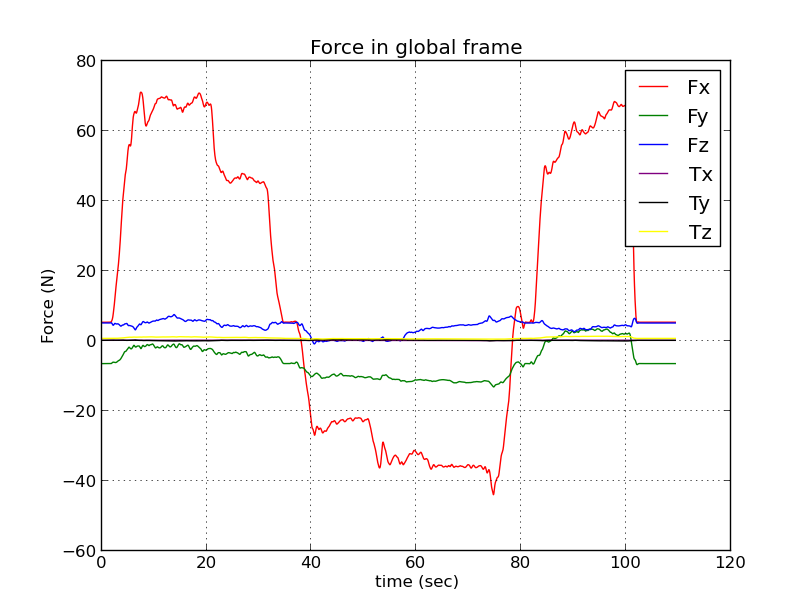
\includegraphics[width = \textwidth ]{high_tor_force} 
    \caption{Filtered data of external wrench detected from F/T sensor}
  \end{subfigure}
  \begin{subfigure}[t]{0.5\textwidth}
    \centering
    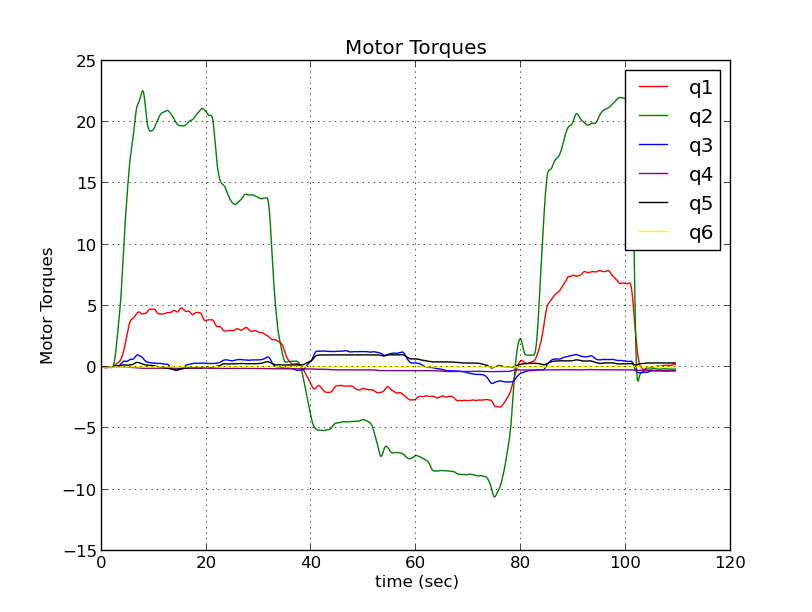
\includegraphics[width = \textwidth ]{high_tor_denso}
    \caption{Filtered data of denso torques}
  \end{subfigure}
  \caption{Sample data of the second joint high torque experiment}
  \label{fig: push result}
\end{figure}

\begin{figure}[H]
  \begin{subfigure}[t]{0.5\textwidth}
    \centering
    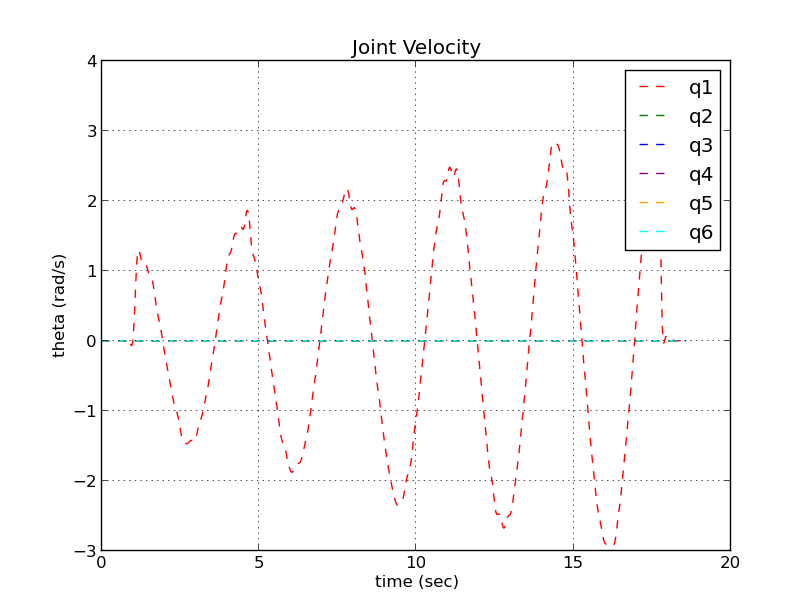
\includegraphics[width = \textwidth ]{high_vel_speed} 
    \caption{Filtered data of joint velocity}
  \end{subfigure}
  \begin{subfigure}[t]{0.5\textwidth}
    \centering
    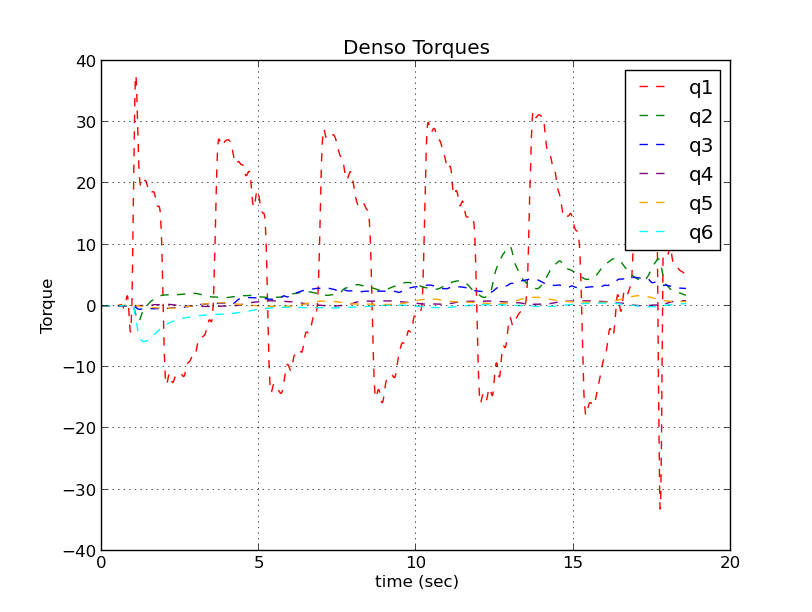
\includegraphics[width = \textwidth ]{high_vel_denso}
    \caption{Filtered data of denso torques}
  \end{subfigure}
  \caption{Sample data of the first joint high velocity experiment}
  \label{fig: fric result}
\end{figure}


\section{Motor Torque Gain Identification}
Based on the setup that has been mentioned in subsection \ref{push exp}, it is known that during the experiment the joints are stationary and hence $\dot{q} = 0$ , $\ddot{q} = 0$. Also since it is not moving, there is no friction effect for the joint. And by using relation in (\ref{denso eq}) and (\ref{tor wrench eq}), equation (\ref{dynamic eq}) can be simplified to: 

\begin{equation}
  K_{denso} \tau_{denso} = - J^{T} F_{ext} + G\left(q \right) \\
\end{equation}

This makes the calibration of $K_{denso}$ becomes more easier to identify as it is a simple linear problem. To get the value of $K_{denso}$, the model is optimized from the data ($\tau_{denso}$, $F_{ext}$) that has been gathered. The optimization is still done by using nelder-mead method. 

The diagram in \fref{fig: tor calibration} shows the plot of $\tau_{denso}$ against $- J^{T} F_{ext}$. The green line represents the experimental data while the black line is the model with optimized parameter $K_{denso}$. As it can be seen, the data is not perfectly linear as what it is supposed to. The reason might be because of the deadzone in motor controller: where errors below some value will be counted as zero. To adjust for this effect, piecewise-linear model can be used to fit the data. Although it will give better results, there are some limitations to the model that make the implementation to be difficult \cite{Nori15}. Hence, simple linear model is still chosen despite the unability to capture the deadzone. 

\begin{figure}[H]
    \centering
    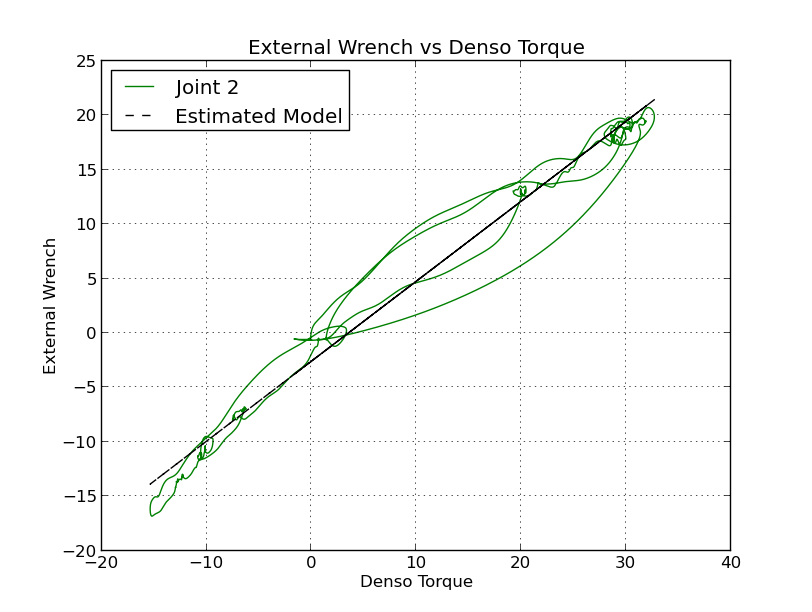
\includegraphics[width = 0.6\textwidth ]{A_6_2}
    \caption{$\tau_{denso}$ vs $- J^{T} F_{ext}$ in high torque experiment for second joint}
    \label{fig: tor calibration}
\end{figure}

The results of the identification can be seen in the table below:
\begin{table}[H]
    \centering
    \begin{tabular}{| c | c |}
    \hline
    Joint & $K_{denso}$             \\ \hline
    1     & 0.9726975092370144      \\ \hline
    2     & 0.7374652918414186      \\ \hline
    3     & 0.5011872413412258      \\ \hline
    4     & 0.17752933989182662     \\ \hline
    5     & 0.22525237806401718     \\ \hline
    6     & 0.08119127531050022     \\ \hline
    \end{tabular}
    \caption{Identification of denso gain parameter}
    \label{table:denso_gain}
\end{table}

\section{Friction Identification}

From section \ref{fric exp} it is known the torques that were exerted during the experiment are coming from friction and inertia torques only. And by choosing the static friction model, the complex equation of \ref{dynamic eq} can be reduced to be a simple dynamic equation of the rigid body:

\begin{equation}
  \tau_{motor} = K_{denso} \tau_{denso} = K_{c} sign\left(\dot{q}\right) + K_{v} \dot{q} + I\ddot{q} \\
\end{equation}

Where $ I $ here is the inertia due to the arm links to the joint. Since all the joints are stationary except for the joint of interest, the inertia should remain constant. This equation is then fitted with the real data to get the three unknown parameters for each joint. Since the optimization now is more complex compared to denso gain identification, the results have to be bounded to make sure that the optimization will not give a wrong answer. Since all of the parameters cannot be negative, the boundary will be: $[K_{c}, K_{v}, I] \geq 0$. the optimization is now done by using Sequential Least SQuares Programming (SLSQP) method provided by SciPy Python. This is because SLSQP can give a boundary condition to the parameters which nelder-mead could not.


Figure below shows the result of optimization to the real plot for the first joint. It can be seen that the plot of the motor torques data are similiar with the static friction diagram(\fref{fig:static fric}) although there are some differences. These differences are most likely due to the inertia that affects the motor torques value. For the second and third joint where inertia is involved, the differences can be seen clearer(\fref{fig:appendix high vel fric}). In contrast, the inertia involved for fourth and sixth joint is very small such that the plot is now look the same as static friction.
 
\begin{figure}[H]
    \centering
    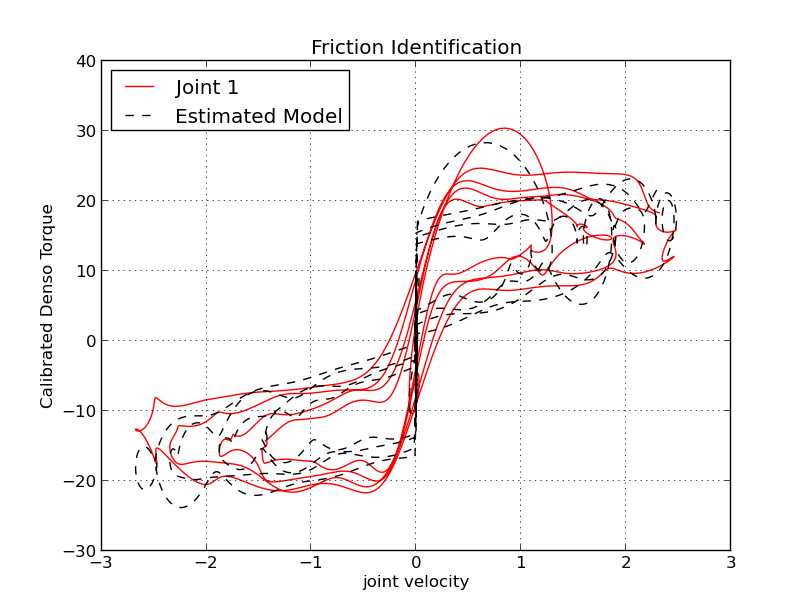
\includegraphics[width = 0.6\textwidth ]{A_7_1}
    \caption{Results for friction identification}
    \label{fig: fric iden}
\end{figure}

The identification results of all parameters for all joints are compiled on the table below: 
\begin{table}[H]
    \centering
    \begin{tabular}{| c | c | c | c |}
    \hline
    Joint & $K_{c}$ & $K_{v}$ & $I$ \\ \hline
    1 & 8.760254598800614   & 3.5593393087764476  & 1.2298914843787225        \\ \hline
    2 & 6.5844162226978975  & 16.631011445572256  & 1.6028523428327148        \\ \hline
    3 & 3.6559073575564893  & 7.240485152284423   & 0.4106659387975339        \\ \hline
    4 & 3.656967856159363   & 2.896319866560603   & 1.204029526208893$e^{-18}$\\ \hline
    5 & 2.5006379799006013  & 3.798780079420939   & 0.12806276310671558       \\ \hline
    6 & 1.336290767286993   & 0.6059130581961736  & 0.0                       \\ \hline
    \end{tabular}
    \caption{Identification of friction torque}
    \label{table:friction}
\end{table}

It is interesting to see that the results for fourth and sixth joints give a very small inertia value. This might be acceptable when considering the setup of the experiments for these two joints. \fref{fig:joint fric setup} show the setup for the fourth and sixth joints during the experiment. Based from this, the inertia will follow inertia of a cylindrical rod with small radius with the centerline as the rotation axis. This configuration will give a smaller value compared to other configurations. Because of this, the optimization will heavily emphasise friction more than the inertia.  

\begin{figure}[H]
  \begin{subfigure}[t]{0.5\textwidth}
    \centering
    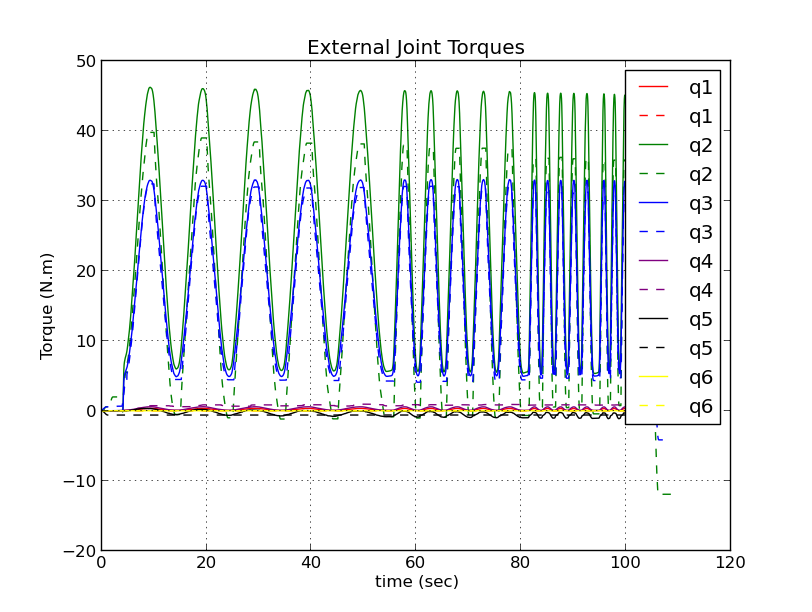
\includegraphics[width = \textwidth ]{fig16} 
    \caption{Fourth joint}
  \end{subfigure}
  \begin{subfigure}[t]{0.5\textwidth}
    \centering
    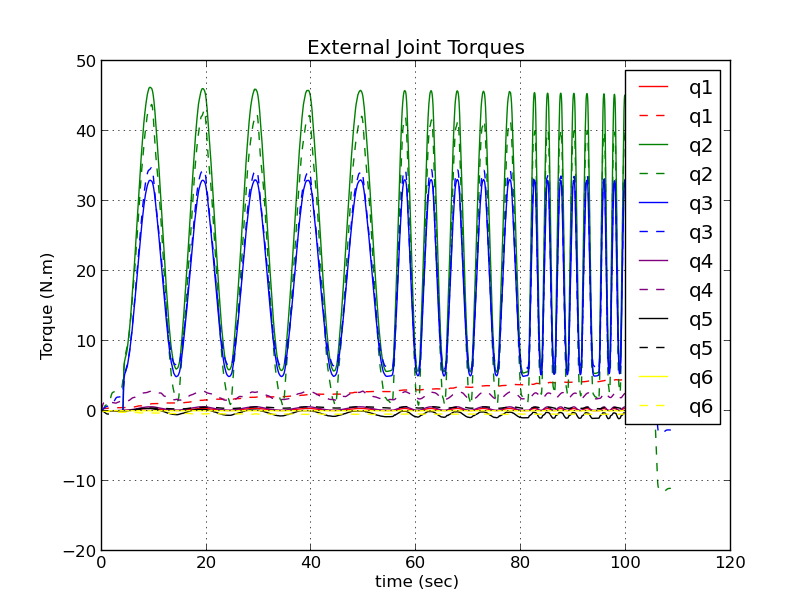
\includegraphics[width = \textwidth ]{fig17}
    \caption{Sixth joint}
  \end{subfigure}
  \caption{Setup of fourth and sixth joints during high velocity experiment}
  \label{fig:joint fric setup}
\end{figure}
